\de{Sei $A$ ein Punkt und sei $k$ ein Kreis durch $A$. Seien $B$ und $C$ zwei weitere Punkte auf $k$. Weiter seien $X$ der Schnittpunkt der Winkelhalbierenden von $\angle ABC$ mit $k$ und $Y$ die Spiegelung von $A$ am Punkt $X$. Sei $D$ der Schnittpunkt der Geraden $YC$ mit $k$. Zeige, dass der Punkt $D$ nicht von der Wahl von $B$ und $C$ auf dem Kreis $k$ abhängt.

\textbf{1. Lösung:} (Paul)
\begin{center}
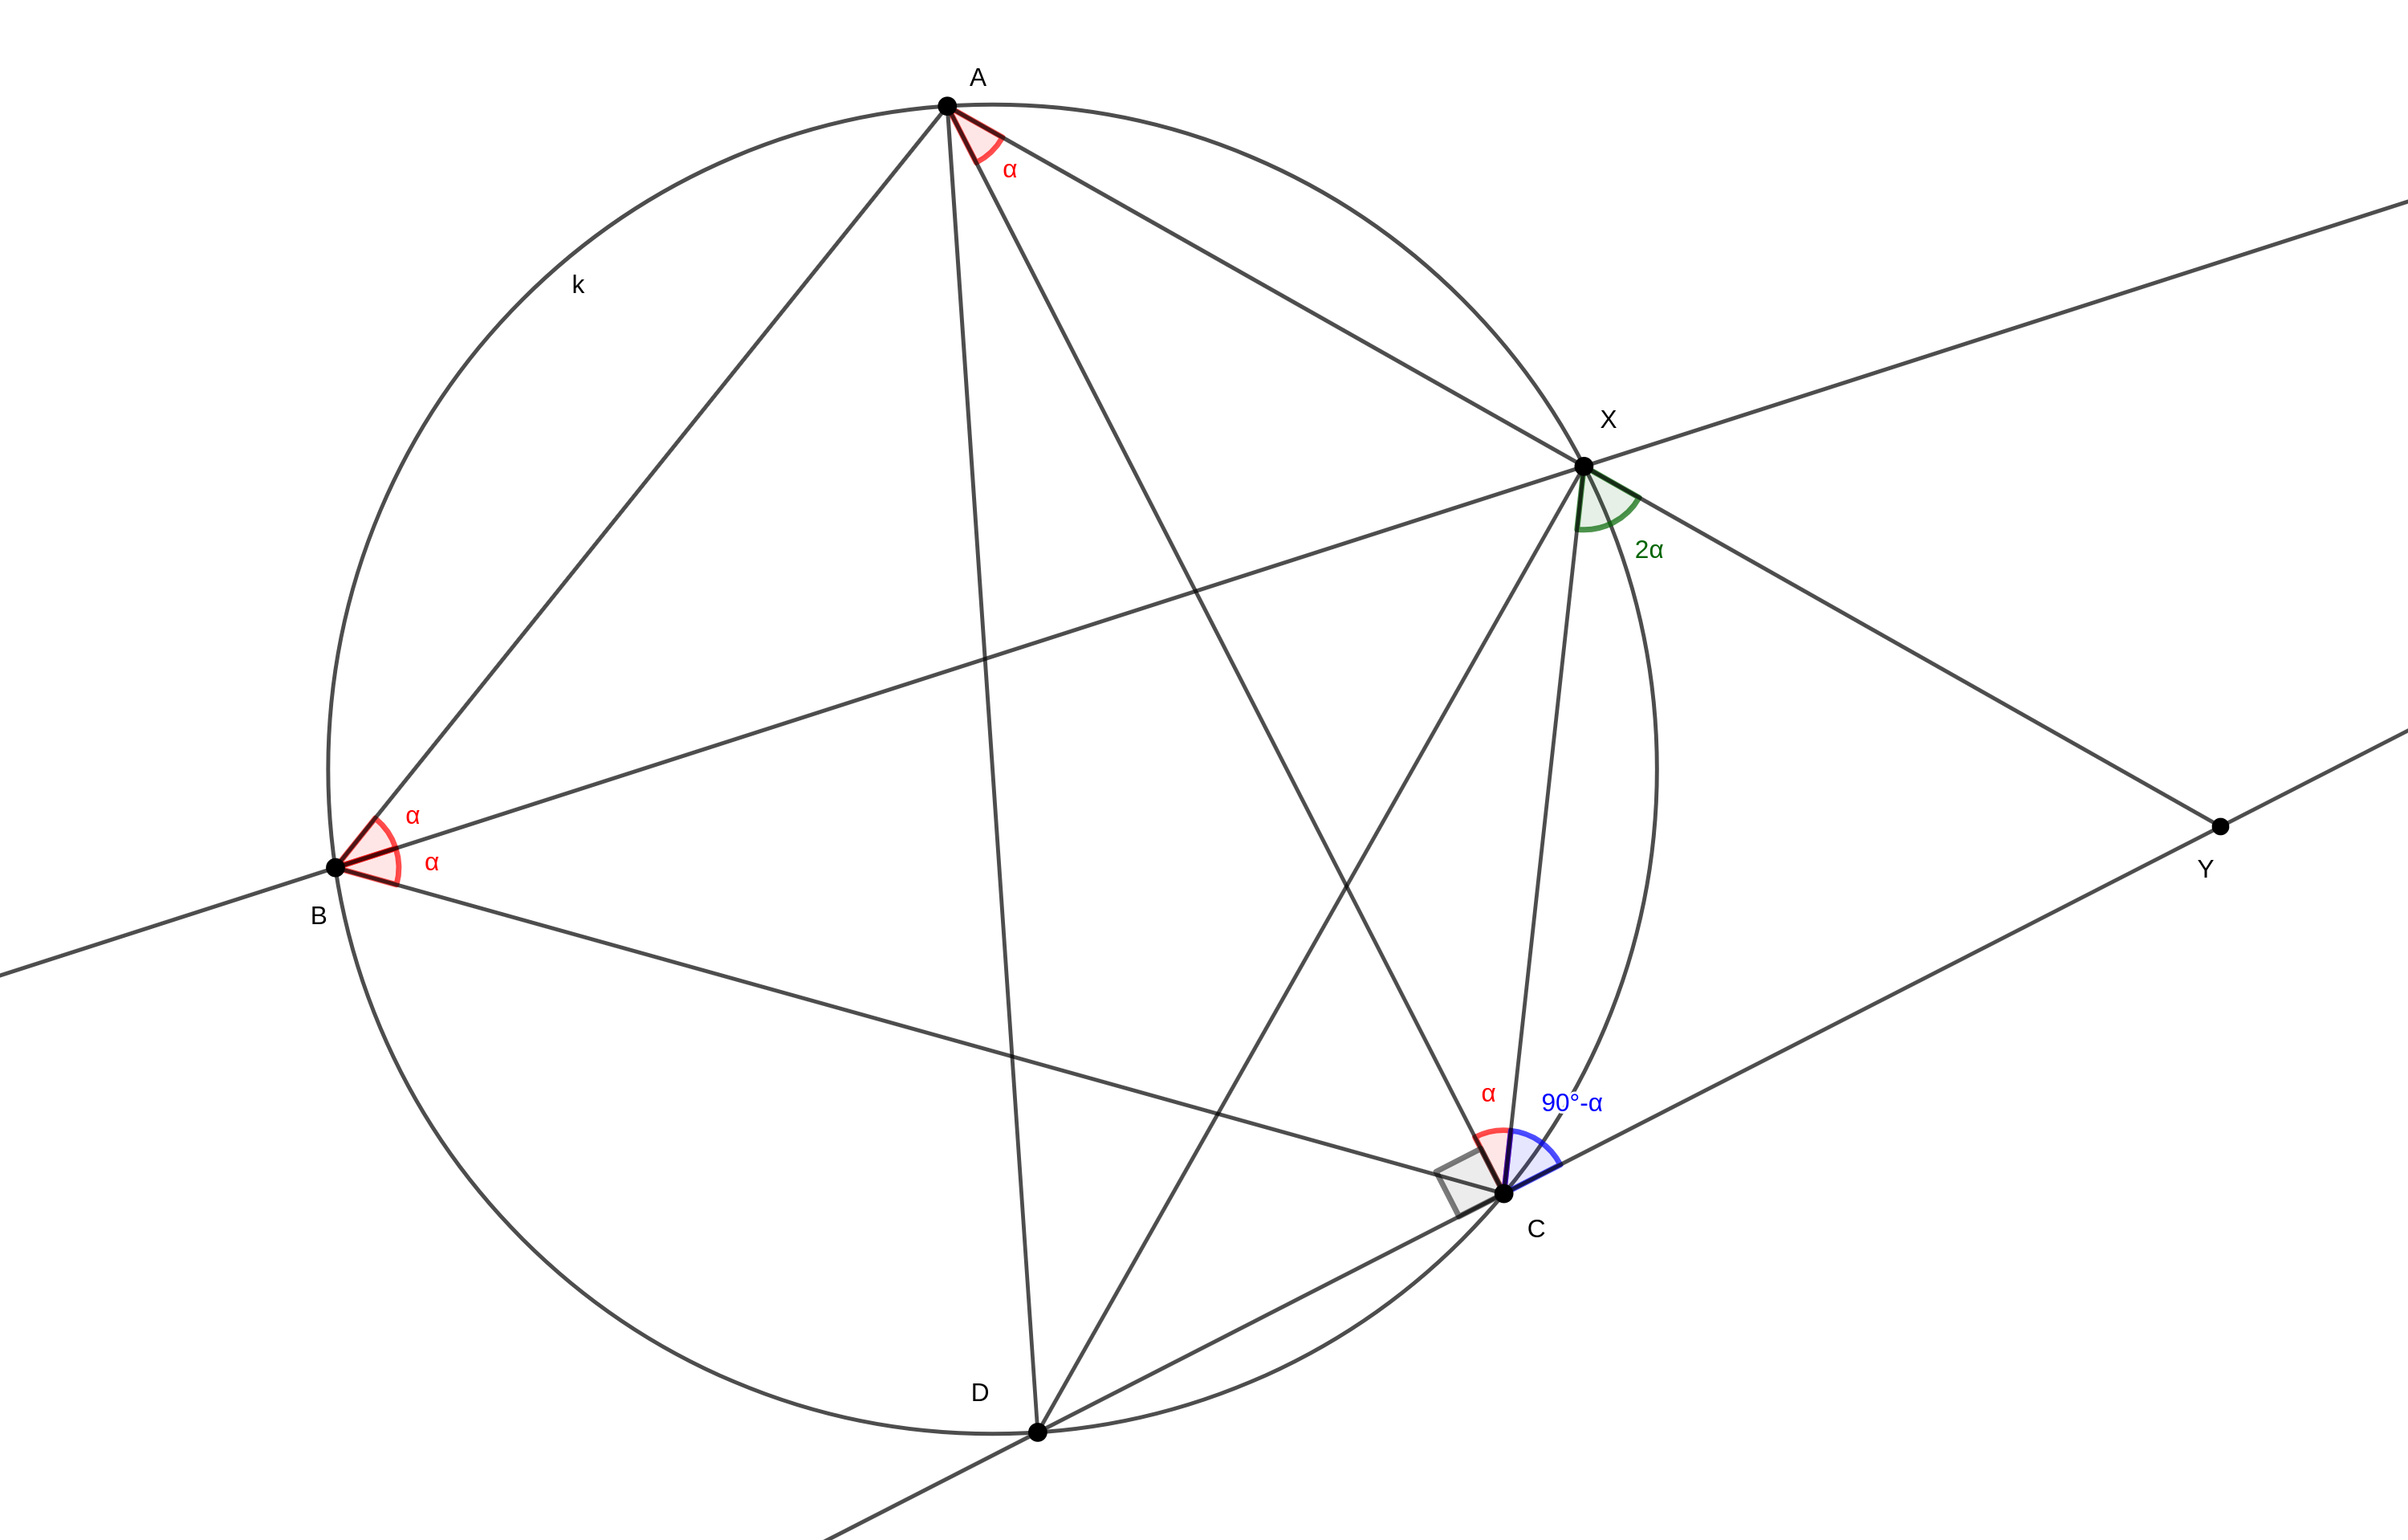
\includegraphics[width=0.8\textwidth]{f1_picture.png}
\end{center}
\vspace{0.8cm}
Sei $\angle ABX = \alpha$. Da $BX$ die Winkelhalbierende von $\angle ABC$ ist, gilt $\angle XBC = \alpha$. Da $ABCX$ ein Sehnenviereck ist, gilt auch $\angle XAC = \angle ACX = \alpha$. Dies bedeutet, dass $AX=XC$. Zusammen mit der Bedingung, dass $Y$ die Spiegelung von $A$ an $X$ ist, ergibt sich $XC=XY$. Wir benutzen nochmal das Sehnenviereck $ABCX$, um
\[
\angle YXC = 180^\circ-\angle CXA = 180^\circ - (180^\circ - \angle ABC) = 2\alpha
\]
zu erhalten. Da $XCY$ gleichschenklig ist, gilt dann $\angle XCY = 90^\circ-\alpha$. Schliesslich  ist
\[
\angle DCA = 180^\circ-\angle ACX - \angle XCY = 180^\circ - \alpha - (90^\circ-\alpha) = 90^\circ.
\]
Dann folgt aus dem Satz von Thales, dass die Strecke $AD$ ein Durchmesser des Kreises $k$ ist. Insbesondere hängt der Ort des Punkts $D$ nur von $A$ und nicht von $B$ oder $C$ ab.
\newpage

\textbf{2. Lösung:} (Arnaud)
Dans la même veine, on observe que 
\[
\angle ADX=\angle ABX=\angle CBX=\angle YDX.
\]
La droite $DX$ est donc la bissectrice de l'angle $\angle ADY$. Or, $X$ se trouve sur $DX$ et $X$ est le milieu de $AY$, donc $DX$ est perpendiculaire à $AY$ (dans le triangle isocèle $ADY$, la bissectrice et la hauteur issues de $D$ se confondent). Autrement dit, $\angle AXD =90^\circ$ et on conclut par le cercle de Thalès que $D$ est simplement le point diamétralement opposé à $A$ sur $k$.

\textbf{3. Lösung:} (David)
Like in the first solution, we immediately get $\angle XAC=\angle XCA$ and we conclude $XA=XC=XY$. So $X$ is the center of a circle going through $A,C,Y$ and with $AY$ as a diameter. By Thales, we get $\angle ACY=90^\circ$ and we conclude.

\textbf{4. Lösung:} (Louis)
Il est bien connu que la bissectrice d'un sommet et la médiatrice du côté opposé se coupent sur le cercle circonscrit (WUM), donc $X$ appartient à la médiatrice du segment $CA$. Si on introduit $M$ le milieu du segment $CA$, on trouve alors que $\angle CMA = 90^{\circ}$ et le triangle $ACY$ est l'image du triangle $AMX$ par une homothétie de centre $A$ et de rapport $2$. On en déduit ainsi que $\angle ACY = \angle AMX = 90^{\circ}$. À partir de là on conclut comme dans les solutions précédentes que $AD$ est un diamètre de $k$.

\textbf{Marking scheme:}
\begin{enumerate}
\item 5P: proving $\angle DCA = 90^\circ$ (or another right angle: $\angle DXA = 90^\circ$ or $\angle DBA = 90^\circ$). At most 2 partial points for this step:
\begin{enumerate}
    \item 2P: for proving either $AX = XC$, $YX=XC$ \textbf{or} $\angle ADX = \angle XDY$
\end{enumerate}
\item 2P: $\angle DCA = 90^\circ$ (or another right angle) $\Rightarrow$ mit Thales fertig 
\end{enumerate}
Bemerkung: Ein Punkt kann abgezogen werden falls der letzte Schritt nicht genau genug erklärt wird.

}